% Provenance (never printed): BCPST year 1 geology (2021), "la carte
% geologique" (reading a map, structures, chronology), union licence
% Sciences de la Terre L1 (cartographie: strike and dip, three-point problem,
% outcrop patterns, DEM and GIS). See sources/outline_sources.md. Pilot
% chapter, 2026-10-22. The region is the series' invented Varden Hills
% (figdata/shared/region.py); every number about it is computed in
% figdata/bachelor-1/varden_maps.py or figdata/bachelor-1/v_rule.py.
\chapter{भूवैज्ञानिक मानचित्र}\label{ch:b1:geological-maps}

एक भूवैज्ञानिक नक्शा-पट्टी, नोटबुक और कंपास-क्लिनोमीटर लेकर नीची पहाड़ियों के बीच से गुज़रता है। अधिकांश ज़मीन
घास, जंगल या जोती हुई खेत है; चट्टान यहाँ-वहाँ ही दिखती है, किसी नाले के किनारे, किसी सड़क की कटान में,
किसी चट्टानी उभार पर। इन बिखरी झलकों से, और भूमि की आकृति से, भूवैज्ञानिक को यह बताना होता है कि
पहाड़ियों के हर वर्ग मीटर के नीचे कौन-सी चट्टान है, परतें किस कोण पर झुकी हैं, वे कहाँ टूटी हैं, और यह
सब किस क्रम में हुआ। परिणाम एक \omterm{def:b1:geological-maps:geological-map}{भूवैज्ञानिक मानचित्र} है: एक सपाट चित्र जो चट्टान के एक त्रि-विमीय पिंड को
कूटबद्ध करता है। यह अध्याय बताता है कि ऐसा मानचित्र कैसे बनता है और कैसे पढ़ा जाता है --- किसी सतह का
\omterm{def:b1:geological-maps:attitude}{अभिविन्यास} कैसे मापा और परिकलित किया जाता है, किसी परत का \omterm{def:b1:geological-maps:geological-map}{बहिर्भाग} वे आकृतियाँ क्यों बनाता है जो वह बनाता
है, और मानचित्र इतिहास कैसे बताता है। इसके उदाहरण एक काल्पनिक पर भूवैज्ञानिक रूप से सुसंगत क्षेत्र, वार्डन
पहाड़ियों, से आते हैं, जो इस पूरी पुस्तक में बार-बार आता है।

\begin{recall}
एक स्थलाकृतिक मानचित्र समोच्च रेखाओं, यानी समान ऊँचाई की रेखाओं, से उच्चावच दिखाता है; उसका पैमाना मानचित्र
की दूरियों को ज़मीन की दूरियों से जोड़ता है (पुस्तक 1, कक्षा 9)। सापेक्ष आयु अध्यारोपण से निकलती है
(परत अपने नीचे की परतों से छोटी होती है, जब तक क्रम उलट न गया हो), आरपार काटने से (जो चट्टान को काटता
है वह उससे छोटा है) और समावेशन से (पुस्तक 1, कक्षा 7)। भ्रंश वह दरार है जिसके साथ दो खंड खिसके हैं
(पुस्तक 1, कक्षा 7); वलनों और भ्रंशों की ज्यामिति \cref{ch:b1:faults-folds-fabrics} का विषय है।
\end{recall}

\section{मानचित्र त्रि-विमीय में एक काट है}\label{sec:b1:geological-maps:cut}

\begin{definition}[भूवैज्ञानिक मानचित्र]\label{def:b1:geological-maps:geological-map}
एक \emph{भूवैज्ञानिक मानचित्र}\index{भूवैज्ञानिक मानचित्र} ज़मीनी सतह के हर बिंदु पर वह शैल-इकाई दिखाता है जो
मिट्टी के नीचे वहाँ पड़ी है, साथ में \emph{संपर्क}\index{संपर्क (भूवैज्ञानिक)} --- वे सतहें जो दो इकाइयों को
अलग करती हैं --- और वे संरचनाएँ (भ्रंश, \omterm{def:b1:geological-maps:fold}{वलन-अक्ष}, परतों के \omterm{def:b1:geological-maps:attitude}{अभिविन्यास}) जो उन्हें प्रभावित करती हैं। एक
\emph{मानचित्र इकाई}\index{मानचित्र इकाई} शैल का वह पिंड है जिसे क्षेत्र में पहचाना और अनुसरित किया जा सके और
जिसे एक रंग में बनाया जाए; उसका \emph{बहिर्भाग}\index{बहिर्भाग} वह क्षेत्र है जहाँ वह सतह पर पड़ा है।
\end{definition}

\begin{definition}[अंकीय उन्नयन मॉडल]\label{def:b1:geological-maps:dem}
एक \emph{अंकीय उन्नयन मॉडल}\index{अंकीय उन्नयन मॉडल} नियमित दूरी वाले बिंदुओं पर ज़मीनी उन्नयनों $z = g(x,y)$
का एक जाल है। एक भौगोलिक सूचना प्रणाली ऐसे जालों को और मानचित्र की अन्य परतों (\omterm{def:b1:geological-maps:geological-map}{संपर्क}, भ्रंश, मापन,
बोरहोल) को एक साझा निर्देशांक-ढाँचे में संग्रहीत करती है और उनके साथ परिकलन करती है।
\end{definition}

\begin{proposition}[एक संपर्क का बहिर्भाग]\label{prop:b1:geological-maps:intersection}
मान लीजिए ज़मीन सतह $z = g(x,y)$ है और एक \omterm{def:b1:geological-maps:geological-map}{संपर्क} सतह $z = c(x,y)$। मानचित्र पर \omterm{def:b1:geological-maps:geological-map}{संपर्क} का अनुरेख वक्र है
\[
  g(x,y) = c(x,y),
\]
जो दो सतहों के प्रतिच्छेद का क्षैतिज समतल पर प्रक्षेप है। \omterm{def:b1:geological-maps:geological-map}{संपर्क} के ऊपर पड़ी इकाई वहाँ \omterm{def:b1:geological-maps:geological-map}{बहिर्भाग} बनाती है
जहाँ $g > c$।
\end{proposition}

\begin{proof}
मानचित्र का एक बिंदु तभी अनुरेख पर होता है जब उस बिंदु पर ज़मीनी सतह \omterm{def:b1:geological-maps:geological-map}{संपर्क} से संबद्ध हो, यानी
$g(x,y) = c(x,y)$। जहाँ $g(x,y) > c(x,y)$ है, वहाँ ज़मीन \omterm{def:b1:geological-maps:geological-map}{संपर्क} के ऊपर है: सतह की चट्टान उस इकाई से है जो
उसके ऊपर पड़ी है।
\end{proof}

\begin{remark}[इस पुस्तक के मानचित्र कैसे बने]\label{rem:b1:geological-maps:computed}
यही ठीक वह तरीका है जिससे एक भौगोलिक सूचना प्रणाली त्रि-विमीय प्रतिरूप से मानचित्र बनाती है: वह \omterm{def:b1:geological-maps:dem}{अंकीय
उन्नयन मॉडल} के जाल पर $g - c$ का मान निकालती है और उन वक्रों का अनुरेख करती है जहाँ वह चिह्न बदलता है।
इस पुस्तक के वार्डन पहाड़ियों के मानचित्र उसी तरह बने, एक ऐसे भूवैज्ञानिक प्रतिरूप से जिसमें हर सतह ज्ञात है।
\end{remark}

\begin{omfigure}
\begin{tikzpicture}
\begin{axis}[axis equal image, xmin=0, xmax=10, ymin=0, ymax=8, width=0.82\linewidth,
  tick label style={font=\scriptsize}, xlabel={पूर्व (km)}, ylabel={उत्तर (km)},
  label style={font=\small}, colormap/blackwhite, enlargelimits=false]
\addplot[matrix plot*, mesh/cols=101, point meta=explicit, shader=interp] table[x=x_km, y=y_km, meta=shade] {figdata/out/bachelor-1-varden_maps-shade.dat};
\addplot[contour, line width=0.25pt, opacity=0.7] table {figdata/out/shared-region-contours.dat};
\addplot[index contour, opacity=0.8] table {figdata/out/shared-region-index-contours.dat};
\addplot[river] table {figdata/out/shared-region-river.dat};
\end{axis}
\end{tikzpicture}

{\small वार्डन पहाड़ियाँ एक \omterm{def:b1:geological-maps:dem}{अंकीय उन्नयन मॉडल} के रूप में: ज़मीन उत्तर-पश्चिम से प्रकाशित, समोच्च रेखाएँ हर
\qty{50}{m} पर (250 और \qty{500}{m} पर मोटी), और नदी, जो पूर्व की ओर बहती है।}
\end{omfigure}

\begin{omfigure}
\begin{tikzpicture}
\begin{axis}[axis equal image, xmin=0, xmax=10, ymin=0, ymax=8, width=0.82\linewidth,
  tick label style={font=\scriptsize}, xlabel={पूर्व (km)}, ylabel={उत्तर (km)},
  label style={font=\small}]
\addplot[lith schist, draw=black, line width=0.3pt, even odd rule] table {figdata/out/shared-region-unit-schist.dat};
\addplot[lith granite, draw=black, line width=0.3pt, even odd rule] table {figdata/out/shared-region-unit-granite.dat};
\addplot[om lith={icsTriassic!35}{om sand}, draw=black, line width=0.3pt, even odd rule] table {figdata/out/shared-region-unit-sandstone.dat};
\addplot[om lith={icsJurassic!40}{om limestone}, draw=black, line width=0.3pt, even odd rule] table {figdata/out/shared-region-unit-limestone.dat};
\addplot[om lith={icsJurassic!15}{om shale}, draw=black, line width=0.3pt, even odd rule] table {figdata/out/shared-region-unit-shale.dat};
\addplot[om lith={icsCretaceous!35}{om limestone}, draw=black, line width=0.3pt, even odd rule] table {figdata/out/shared-region-unit-chalk.dat};
% the fault is drawn before the alluvium: the younger alluvial floor conceals it
\addplot[normal fault] table {figdata/out/shared-region-fault.dat};
\addplot[lith alluvium, draw=black, line width=0.3pt, even odd rule] table {figdata/out/shared-region-unit-alluvium.dat};
\addplot[contour, opacity=0.55] table {figdata/out/shared-region-contours.dat};
\addplot[river] table {figdata/out/shared-region-river.dat};
\pic at (axis cs:4.3,6.6) {strikedip={350.6}{12}};
\pic at (axis cs:2.2,6.6) {strikedip={189.3}{12}};
\pic at (axis cs:8.6,1.4) {northarrow};
\fill[black] (axis cs:6.6,0.35) rectangle (axis cs:7.1,0.5);
\fill[white] (axis cs:7.1,0.35) rectangle (axis cs:7.6,0.5);
\fill[black] (axis cs:7.6,0.35) rectangle (axis cs:8.1,0.5);
\fill[white] (axis cs:8.1,0.35) rectangle (axis cs:8.6,0.5);
\draw[black, line width=0.4pt] (axis cs:6.6,0.35) rectangle (axis cs:8.6,0.5);
\node[font=\footnotesize, above, inner sep=1.5pt, fill=white, fill opacity=0.8, text opacity=1] at (axis cs:7.6,0.5) {\qty{2}{km}};
\end{axis}
\end{tikzpicture}

\smallskip
\begin{tikzpicture}[font=\footnotesize]
\matrix[column sep=7pt, row sep=3pt, matrix of nodes, nodes={anchor=west}] {
  \tikz\draw[black!60, line width=0.4pt, lith alluvium] (0,0) rectangle (0.7,0.32); & जलोढ़ (क्वाटरनरी) &
  \tikz\draw[black!60, line width=0.4pt, om lith={icsCretaceous!35}{om limestone}] (0,0) rectangle (0.7,0.32); & खड़िया (क्रेटेशियस, 90 Ma) \\
  \tikz\draw[black!60, line width=0.4pt, om lith={icsJurassic!15}{om shale}] (0,0) rectangle (0.7,0.32); & शेल (जुरैसिक, 165 Ma) &
  \tikz\draw[black!60, line width=0.4pt, om lith={icsJurassic!40}{om limestone}] (0,0) rectangle (0.7,0.32); & चूना पत्थर (जुरैसिक, 180 Ma) \\
  \tikz\draw[black!60, line width=0.4pt, om lith={icsTriassic!35}{om sand}] (0,0) rectangle (0.7,0.32); & बलुआ पत्थर (ट्राइऐसिक, 245 Ma) &
  \tikz\draw[black!60, line width=0.4pt, lith granite] (0,0) rectangle (0.7,0.32); & ग्रेनाइट (310 Ma) \\
  \tikz\draw[black!60, line width=0.4pt, lith schist] (0,0) rectangle (0.7,0.32); & शिस्ट (480 Ma) &
  \tikz\draw[normal fault] (0,0.16) -- (0.9,0.16); & सामान्य भ्रंश (खड़े निशान अवनत ओर) \\
};
\end{tikzpicture}

{\small वार्डन पहाड़ियों का \omterm{def:b1:geological-maps:geological-map}{भूवैज्ञानिक मानचित्र}, समोच्च रेखाओं, नदी, दो मापे गए अभिविन्यासों (\omterm{def:b1:geological-maps:attitude}{स्ट्राइक} रेखा और
नति-निशान, \omterm{def:b1:geological-maps:attitude}{नति} डिग्री में) और उपाख्यान के साथ। इकाइयों की आयु उस क्षेत्र की इकाइयों की है; भ्रंश घाटी-तली की
अपेक्षाकृत नई जलोढ़ के नीचे छिपा है।}
\end{omfigure}

\section{एक समतल का अभिविन्यास}

\begin{definition}[स्ट्राइक, नति और नति-दिशा]\label{def:b1:geological-maps:attitude}
मान लीजिए एक भूवैज्ञानिक सतह --- एक शय्या-तल, एक \omterm{def:b1:geological-maps:geological-map}{संपर्क}, एक भ्रंश --- स्थानीय रूप से एक समतल है। उसका
\emph{स्ट्राइक}\index{स्ट्राइक} उन क्षैतिज रेखाओं की दिशा है जो उसमें हैं, दिगंश के रूप में दी गई (उत्तर से
घड़ी की दिशा में डिग्री)। उसकी \emph{नति}\index{नति} $\delta$ समतल और क्षैतिज के बीच का कोण है, जो स्ट्राइक के
लंबवत ऊर्ध्वाधर तल में मापा जाता है, $0 \le \delta \le \ang{90}$। उसकी \emph{नति-दिशा}\index{नति-दिशा} $\alpha$
समतल की सबसे खड़ी अधोमुखी रेखा का दिगंश है। साथ मिलकर वे समतल का \emph{अभिविन्यास}\index{अभिविन्यास (समतल का)}
बनाते हैं, जो नति-दिशा/नति के रूप में लिखा जाता है, जैसे $080/12$।
\end{definition}

\begin{notation}[दाएँ-हाथ के नियम से स्ट्राइक]\label{not:b1:geological-maps:rhr}
\omterm{def:b1:geological-maps:attitude}{स्ट्राइक} को दो विपरीत दिशाओं में पढ़ा जा सकता है। \emph{दाएँ-हाथ का नियम} वह दिशा चुनता है जिसमें, \omterm{def:b1:geological-maps:attitude}{स्ट्राइक} के
अनुदिश देखने वाले प्रेक्षक के लिए, समतल दाईं ओर नीचे झुकता है: \omterm{def:b1:geological-maps:attitude}{स्ट्राइक} $= \alpha - \ang{90}$ (\ang{360} के मॉड्यूलो)।
मानचित्र पर चिह्न एक \omterm{def:b1:geological-maps:attitude}{स्ट्राइक} रेखा है जिस पर \omterm{def:b1:geological-maps:attitude}{नति} की दिशा में इंगित एक छोटा निशान है, और \omterm{def:b1:geological-maps:attitude}{नति} से अंकित।
\end{notation}

\begin{omfigure}
\tdplotsetmaincoords{65}{125}
\begin{tikzpicture}[tdplot_main_coords, font=\small, scale=1.05]
  % the horizontal plane
  \fill[omSea!50] (-2.2,-1.6,0) -- (2.2,-1.6,0) -- (2.2,1.6,0) -- (-2.2,1.6,0) -- cycle;
  \draw[black!40] (-2.2,-1.6,0) -- (2.2,-1.6,0) -- (2.2,1.6,0) -- (-2.2,1.6,0) -- cycle;
  % the dipping plane: strike along y (north), dipping east (+x) at 30 degrees
  \fill[omLithLime!80, opacity=0.85] (-0.0,-1.6,0) -- (-0.0,1.6,0) -- (2.2,1.6,-1.27) -- (2.2,-1.6,-1.27) -- cycle;
  \draw[black!60] (0,-1.6,0) -- (0,1.6,0) -- (2.2,1.6,-1.27) -- (2.2,-1.6,-1.27) -- cycle;
  % strike line (horizontal, in both planes)
  \draw[omThm, line width=1.1pt] (0,-1.6,0) -- (0,1.6,0);
  % dip line and the horizontal below it, with the dip angle
  \draw[omDef, line width=1.1pt, -{Stealth[length=2.4mm]}] (0,0,0) -- (2.2,0,-1.27);
  \draw[black!60, densely dashed] (0,0,0) -- (2.2,0,0);
  \draw[black!60, densely dashed] (2.2,0,0) -- (2.2,0,-1.27);
  \draw[black] plot[domain=0:30, samples=16, variable=\t] ({0.8*cos(\t)}, 0, {-0.8*sin(\t)});
  \node[font=\footnotesize] at (1.05,0,-0.22) {$\delta$};
  % north arrow on the horizontal plane
  \draw[black, -{Stealth[length=2mm]}] (-1.8,-1.2,0) -- (-1.8,-0.3,0);
  \node[font=\footnotesize] at (-1.8,-0.05,0) {\omnameCompassN};
\end{tikzpicture}
\begin{tikzpicture}[font=\small]
  \node[align=left, anchor=west, text width=5.2cm] at (0,0) {%
    \textcolor{omThm}{\rule[0.5ex]{0.6cm}{1.1pt}} स्ट्राइक: समतल की एक क्षैतिज रेखा;\\[3pt]
    \textcolor{omDef}{\rule[0.5ex]{0.6cm}{1.1pt}} समतल पर सबसे खड़ी रेखा, जिसका दिगंश नति-दिशा है;\\[3pt]
    नति इस रेखा और क्षैतिज (बिंदुरेखा) के बीच का कोण है।};
\end{tikzpicture}

{\small एक समतल जो उत्तर की ओर \omterm{def:b1:geological-maps:attitude}{स्ट्राइक} करता है और पूर्व की ओर \ang{30} झुकता है (\omterm{def:b1:geological-maps:attitude}{अभिविन्यास}
$090/30$), अपनी \omterm{def:b1:geological-maps:attitude}{स्ट्राइक} रेखा के साथ एक क्षैतिज समतल को काटता हुआ। पैमाने पर नहीं।}
\end{omfigure}

\begin{proposition}[झुके हुए समतल का समीकरण]\label{prop:b1:geological-maps:plane}
$x$ पूर्व की ओर, $y$ उत्तर की ओर और $z$ ऊपर की ओर लेने पर, \omterm{def:b1:geological-maps:attitude}{नति-दिशा} $\alpha$ और \omterm{def:b1:geological-maps:attitude}{नति} $\delta$ वाला, बिंदु $(x_0, y_0, z_0)$ से होकर जाने वाला समतल है
\[
  z = z_0 - \tan\delta\,\bigl[(x - x_0)\sin\alpha + (y - y_0)\cos\alpha\bigr].
\]
\end{proposition}

\begin{proof}
\omterm{def:b1:geological-maps:attitude}{नति-दिशा} की ओर इंगित क्षैतिज इकाई सदिश है $\vec u = (\sin\alpha, \cos\alpha, 0)$ (दिगंश उत्तर से, यानी
$y$ अक्ष से, पूर्व की ओर, यानी $x$ अक्ष की ओर मापा जाता है)। \omterm{def:b1:geological-maps:attitude}{स्ट्राइक} के अनुदिश, $\vec u$ के लंबवत, समतल
क्षैतिज है; $\vec u$ के अनुदिश वह क्षैतिज दूरी की प्रति इकाई $\tan\delta$ नीचे उतरता है। बिंदु $(x_0, y_0)$
से गुज़रने वाली \omterm{def:b1:geological-maps:attitude}{स्ट्राइक} रेखा से किसी बिंदु की क्षैतिज दूरी, जो \omterm{def:b1:geological-maps:attitude}{नति} की दिशा में धनात्मक गिनी जाती है, $(x-x_0)\sin\alpha + (y-y_0)\cos\alpha$ है, जिससे सूत्र मिलता है।
\end{proof}

\begin{theorem}[तीन बिंदुओं से अभिविन्यास]\label{thm:b1:geological-maps:three-point}
मान लीजिए $P_1, P_2, P_3$ एक समतल के तीन असरेखीय बिंदु हैं, और
$\vec n = \overrightarrow{P_1P_2} \times \overrightarrow{P_1P_3} =
(n_x, n_y, n_z)$, $n_z > 0$ के साथ चुना गया (अन्यथा $\vec n$ को $-\vec n$ से बदलिए)। तब समतल की \omterm{def:b1:geological-maps:attitude}{नति} और
\omterm{def:b1:geological-maps:attitude}{नति-दिशा} हैं
\[
  \delta = \arccos\frac{n_z}{\|\vec n\|}, \qquad
  \alpha = \text{क्षैतिज सदिश का दिगंश } (n_x, n_y),
\]
यानी वह कोण $\alpha \in [\ang{0}, \ang{360})$ जिसके लिए
$\sin\alpha = n_x/\sqrt{n_x^2+n_y^2}$ और $\cos\alpha = n_y/\sqrt{n_x^2+n_y^2}$ है (समतल क्षैतिज है यदि
$n_x = n_y = 0$)।
\end{theorem}

\begin{proof}
$\vec n$ समतल के दो स्वतंत्र सदिशों के लंबवत है, अतः उसके अभिलंब है। \omterm{def:b1:geological-maps:attitude}{नति} समतल और क्षैतिज के बीच का कोण है,
जो उनके अभिलंबों $\vec n$ और ऊर्ध्वाधर $\vec k$ के बीच के कोण के बराबर है: $\cos\delta = \vec n \cdot \vec k / \|\vec n\| = n_z/\|\vec n\|$। \cref{prop:b1:geological-maps:plane} से समतल
$z = \text{स्थिरांक} -
\tan\delta\,(x\sin\alpha + y\cos\alpha)$ है, अर्थात्
$\tan\delta\sin\alpha\,x + \tan\delta\cos\alpha\,y + z = \text{स्थिरांक}$; उसका ऊर्ध्व अभिलंब $(\tan\delta\sin\alpha,
\tan\delta\cos\alpha, 1)$ के समानुपाती है, जिसका क्षैतिज भाग \omterm{def:b1:geological-maps:attitude}{नति-दिशा} $\alpha$ की ओर इंगित करता है। चूँकि $\vec n$ इस
अभिलंब का धनात्मक गुणज है, $(n_x, n_y)$ भी \omterm{def:b1:geological-maps:attitude}{नति-दिशा} की ओर इंगित करता है।
\end{proof}

\begin{method}[तीन-बिंदु समस्या]\label{met:b1:geological-maps:three-point}
तीन बोरहोलों में मिले (या तीन बहिर्भागों पर देखे गए) एक \omterm{def:b1:geological-maps:geological-map}{संपर्क} का \omterm{def:b1:geological-maps:attitude}{अभिविन्यास} ज्ञात करने के लिए:
\begin{enumerate}
  \item हर बोरहोल के लिए \omterm{def:b1:geological-maps:geological-map}{संपर्क} का उन्नयन लीजिए: ज़मीन का उन्नयन घटा वह गहराई जिस पर \omterm{def:b1:geological-maps:geological-map}{संपर्क} मिला;
  \item तीन बिंदुओं $P_i = (x_i, y_i, z_i)$ को मीटर में लिखिए, $x$ पूर्व, $y$ उत्तर;
  \item $\vec n = \overrightarrow{P_1P_2} \times
        \overrightarrow{P_1P_3}$ परिकलित कीजिए और $n_z$ को धनात्मक बनाइए;
  \item \cref{thm:b1:geological-maps:three-point} लगाइए; \omterm{def:b1:geological-maps:attitude}{अभिविन्यास} को \omterm{def:b1:geological-maps:attitude}{नति-दिशा}/\omterm{def:b1:geological-maps:attitude}{नति} के रूप में दीजिए और, यदि पूछा
        जाए, दाएँ-हाथ के नियम से \omterm{def:b1:geological-maps:attitude}{स्ट्राइक}।
\end{enumerate}
कागज़ पर वही समस्या संरचना समोच्चों से हल होती है: सबसे ऊँचे और सबसे नीचे बिंदुओं को जोड़ने वाली रेखा पर,
अनुपात से, तीसरे बिंदु के उन्नयन वाला बिंदु खोजिए; इन दो समान-उन्नयन बिंदुओं से गुज़रने वाली रेखा एक \omterm{def:b1:geological-maps:attitude}{स्ट्राइक}
रेखा है; \omterm{def:b1:geological-maps:attitude}{नति} दो समांतर \omterm{def:b1:geological-maps:attitude}{स्ट्राइक} रेखाओं के बीच के उन्नयन-अंतर और उनकी दूरी से निकलती है।
\end{method}

\begin{example}[वार्डन अपनति की पूर्वी भुजा]\label{ex:b1:geological-maps:east}
% computed in figdata/bachelor-1/varden_maps.py (boreholes E1-E3)
तीन बोरहोल, E1 $(4000, 6000)$ पर, E2 $(4600, 7200)$ पर और E3 $(5100, 6400)$ पर (मीटर में मानचित्र के दक्षिण-पश्चिम
कोने से पूर्व और उत्तर), चूना-पत्थर के आधार को उन्नयनों $174$, $4$ और $\qty{-74}{m}$ पर पाते हैं। तब
$\overrightarrow{P_1P_2} = (600, 1200, -170)$,
$\overrightarrow{P_1P_3} = (1100, 400, -248)$; उनका सदिश गुणनफल
$(-229\,600, -38\,200, -1\,080\,000)$ है, जो नीचे की ओर इंगित करता है, अतः
\[
  \vec n = (229\,600,\ 38\,200,\ 1\,080\,000).
\]
अतः $\cos\delta = 1\,080\,000/\|\vec n\| \approx
0.9776$, $\delta \approx \ang{12.2}$, और \omterm{def:b1:geological-maps:attitude}{नति-दिशा} $(229\,600, 38\,200)$ का दिगंश है, $\alpha \approx \ang{80.6}$:
\omterm{def:b1:geological-maps:attitude}{अभिविन्यास} $081/12$ है, दाएँ-हाथ के नियम से \omterm{def:b1:geological-maps:attitude}{स्ट्राइक} $\ang{351}$। चूना-पत्थर का आधार हल्का पूर्व-उत्तर-पूर्व
की ओर झुकता है।
\end{example}

\section{बहिर्भाग के प्रारूप}

\begin{proposition}[क्षैतिज और ऊर्ध्वाधर संपर्क]\label{prop:b1:geological-maps:hv}
एक क्षैतिज \omterm{def:b1:geological-maps:geological-map}{संपर्क} का अनुरेख उसकी ऊँचाई की समोच्च रेखा का अनुसरण करता है। एक ऊर्ध्वाधर \omterm{def:b1:geological-maps:geological-map}{संपर्क} का अनुरेख मानचित्र पर
एक सीधी रेखा है, उच्चावच चाहे जैसा हो।
\end{proposition}

\begin{proof}
$c(x,y) = z_0$ के लिए अनुरेख $g(x,y) = z_0$, यानी समोच्च $z_0$ है
(\cref{prop:b1:geological-maps:intersection})। एक ऊर्ध्वाधर समतल उन बिंदुओं का समुच्चय है जिनकी क्षैतिज स्थिति
एक सीधी रेखा पर है, किसी भी उन्नयन पर; मानचित्र पर उसका अनुरेख वही रेखा है।
\end{proof}

\begin{theorem}[V-नियम]\label{thm:b1:geological-maps:v-rule}
एक समतल \omterm{def:b1:geological-maps:geological-map}{संपर्क} एक ऐसी घाटी को काटता है जिसका तल प्रवाह की दिशा में प्रवणता $s > 0$ से नीचे उतरता है। मान लीजिए
$a$ \omterm{def:b1:geological-maps:geological-map}{संपर्क} की प्रवाह की दिशा में प्रकट \omterm{def:b1:geological-maps:attitude}{नति} की स्पर्शज्या है ($a > 0$ यदि वह प्रवाह की दिशा में झुकता है, $a < 0$ यदि
वह प्रवाह के विपरीत झुकता है, $a = 0$ यदि क्षैतिज है)। तब \omterm{def:b1:geological-maps:geological-map}{बहिर्भाग} का अनुरेख एक V बनाता है जिसका शीर्ष घाटी
के तल पर है, और
\begin{itemize}
  \item यदि $a > s$ तो V \emph{प्रवाह की ओर} इंगित करता है: \omterm{def:b1:geological-maps:geological-map}{संपर्क} प्रवाह की दिशा में इतनी तीखी \omterm{def:b1:geological-maps:attitude}{नति} से झुकता है
        जितनी तीखी घाटी का तल नीचे उतरता है;
  \item यदि $a < s$ तो V \emph{प्रवाह के विपरीत} इंगित करता है: \omterm{def:b1:geological-maps:geological-map}{संपर्क} क्षैतिज है, प्रवाह के विपरीत झुकता है, या
        प्रवाह की दिशा में तल से कम तीखी \omterm{def:b1:geological-maps:attitude}{नति} से झुकता है।
\end{itemize}
एक ऊर्ध्वाधर \omterm{def:b1:geological-maps:geological-map}{संपर्क} कोई V नहीं बनाता।
\end{theorem}

\begin{proof}
मान लीजिए $\xi$ घाटी के तल के अनुदिश प्रवाह की दिशा में मापी गई दूरी है। तल उन्नयन $z_g(\xi) = z_0 - s\xi$ पर है;
घाटी के अनुदिश ऊर्ध्वाधर काट में \omterm{def:b1:geological-maps:geological-map}{संपर्क} $z_c(\xi) = c - a\xi$ पर है। तल पर अनुरेख वहाँ है जहाँ $z_g = z_c$:
\[
  \xi_{\text{तल}} = \frac{c - z_0}{a - s}.
\]
घाटी के एक किनारे पर, जो तल से $h > 0$ ऊँचा है और घाटी के स्रोत से उसी दूरी पर है, ज़मीन $z_0 - s\xi + h$ पर है,
अतः अनुरेख वहाँ है जहाँ $c - a\xi = z_0 - s\xi + h$:
\[
  \xi_{\text{किनारा}} = \frac{c - z_0 - h}{a - s}, \qquad
  \xi_{\text{तल}} - \xi_{\text{किनारा}} = \frac{h}{a - s}.
\]
यदि $a > s$, तो अनुरेख तल पर किनारों की तुलना में अधिक प्रवाह की ओर स्थित है: V प्रवाह की ओर इंगित करता है। यदि
$a < s$, तो उल्टा। एक ऊर्ध्वाधर \omterm{def:b1:geological-maps:geological-map}{संपर्क} तल और किनारों को एक ही $\xi$ पर काटता है।
\end{proof}

\begin{omfigure}
\begin{tikzpicture}
\pgfplotsset{vpanel/.style={axis equal image, xmin=-1, xmax=1, ymin=0, ymax=2,
  width=4.1cm, ticks=none, axis line style={black!50}, clip=true,
  title style={font=\footnotesize, align=center, yshift=-2pt}}}
\begin{axis}[vpanel, at={(0cm,0cm)}, title={क्षैतिज}]
\addplot[contour, opacity=0.8] table {figdata/out/bachelor-1-v_rule-contours.dat};
\addplot[omThm, line width=1.2pt] table {figdata/out/bachelor-1-v_rule-h.dat};
\addplot[river, -{Stealth[length=1.6mm]}] coordinates {(0,0.05) (0,1.95)};
\end{axis}
\begin{axis}[vpanel, at={(3.15cm,0cm)}, title={प्रवाह के विपरीत\\ झुकता हुआ}]
\addplot[contour, opacity=0.8] table {figdata/out/bachelor-1-v_rule-contours.dat};
\addplot[omThm, line width=1.2pt] table {figdata/out/bachelor-1-v_rule-u.dat};
\addplot[river, -{Stealth[length=1.6mm]}] coordinates {(0,0.05) (0,1.95)};
\end{axis}
\begin{axis}[vpanel, at={(6.3cm,0cm)}, title={प्रवाह की ओर,\\ तल से धीमा}]
\addplot[contour, opacity=0.8] table {figdata/out/bachelor-1-v_rule-contours.dat};
\addplot[omThm, line width=1.2pt] table {figdata/out/bachelor-1-v_rule-g.dat};
\addplot[river, -{Stealth[length=1.6mm]}] coordinates {(0,0.05) (0,1.95)};
\end{axis}
\begin{axis}[vpanel, at={(9.45cm,0cm)}, title={प्रवाह की ओर,\\ तल से तीखा}]
\addplot[contour, opacity=0.8] table {figdata/out/bachelor-1-v_rule-contours.dat};
\addplot[omThm, line width=1.2pt] table {figdata/out/bachelor-1-v_rule-d.dat};
\addplot[river, -{Stealth[length=1.6mm]}] coordinates {(0,0.05) (0,1.95)};
\end{axis}
\end{tikzpicture}

{\small V-नियम का परिकलित रूप। हर पैनल में एक नदी (नीला तीर) घाटी के नीचे उत्तर की ओर बहती है, जिसकी
समोच्च रेखाएँ (हर \qty{10}{m} पर) ऊपर की ओर, यानी प्रवाह के विपरीत, इंगित करती हैं; पूर्व-पश्चिम \omterm{def:b1:geological-maps:attitude}{स्ट्राइक} वाला
एक \omterm{def:b1:geological-maps:geological-map}{संपर्क} लाल रंग में अनुरेखित है। क्षैतिज होने पर वह समोच्च रेखाओं का अनुसरण करता है; प्रवाह के विपरीत झुकने पर,
या प्रवाह की दिशा में तल से कम तीखी \omterm{def:b1:geological-maps:attitude}{नति} से झुकने पर, वह प्रवाह के विपरीत इंगित करता V बनाता है; प्रवाह की
दिशा में तल से अधिक तीखी \omterm{def:b1:geological-maps:attitude}{नति} (यहाँ \ang{10}) से झुकने पर, प्रवाह की ओर इंगित करता V। एक ऊर्ध्वाधर \omterm{def:b1:geological-maps:geological-map}{संपर्क} सीधा
आर-पार जाता।}
\end{omfigure}

\begin{remark}[बहिर्भाग की चौड़ाई]\label{rem:b1:geological-maps:width}
एक इकाई के \omterm{def:b1:geological-maps:geological-map}{बहिर्भाग} की चौड़ाई उसकी मोटाई, उसकी \omterm{def:b1:geological-maps:attitude}{नति} और ज़मीन की ढलान पर निर्भर करती है: एक पतली परत जो
ढलान की उसी दिशा में झुकती है, एक विस्तृत क्षेत्र में \omterm{def:b1:geological-maps:geological-map}{बहिर्भाग} बना सकती है। मोटाई एक मानचित्र और एक
अनुप्रस्थ काट से \cref{ch:b1:cross-sections} में परिकलित की जाती है।
\end{remark}

\section{मानचित्र पर वलन, भ्रंश, अंतर्वेधन और असंगतियाँ}

\begin{definition}[अपनति और अभिनति]\label{def:b1:geological-maps:fold}
एक \emph{वलन}\index{वलन} एक बार समतल रही परतों का मोड़ है। एक
\emph{अपनति}\index{अपनति} ऐसा वलन है जिसकी परतें ऊपर की ओर उत्तल हैं (ऊर्ध्व वलन); एक
\emph{अभिनति}\index{अभिनति} ऐसा वलन है जिसकी परतें ऊपर की ओर अवतल हैं (अधोमुखी वलन)। वलन के दो पार्श्व उसकी
भुजाएँ हैं; उसका \emph{वलन-अक्ष}\index{वलन-अक्ष} वह रेखा है जिसके अनुदिश परतें सबसे अधिक मुड़ती हैं, और
अक्ष जब क्षैतिज न हो तो नमन करता है। वलन-अक्ष जैसी रेखा उसके क्षैतिज प्रक्षेप का
दिगंश, जो नीचे की दिशा में लिया जाता है, और उसके नमन, वह कोण जो वह क्षैतिज से बनाती है, से
स्थित की जाती है (\cref{ch:b1:field-lab-methods-1})। त्रि-विमीय में वलन की ज्यामिति \cref{ch:b1:faults-folds-fabrics}
का विषय है।
\end{definition}

\begin{proposition}[वलन के प्रारूप]\label{prop:b1:geological-maps:folds}
अपरदित वलित परतों के एक मानचित्र पर, एक \omterm{def:b1:geological-maps:fold}{अपनति} अपने क्रोड में सबसे पुरानी इकाइयाँ और दोनों ओर बाहर की ओर
छोटी इकाइयाँ दिखाती है; एक \omterm{def:b1:geological-maps:fold}{अभिनति} अपने क्रोड में सबसे नई इकाई दिखाती है। यदि \omterm{def:b1:geological-maps:fold}{वलन-अक्ष} नमन करता है, तो
\omterm{def:b1:geological-maps:geological-map}{बहिर्भाग} \omterm{def:b1:geological-maps:fold}{वलन} के चारों ओर बंद हो जाते हैं: \omterm{def:b1:geological-maps:fold}{अपनति} का बंद होना नमन की दिशा में इंगित करता है, और \omterm{def:b1:geological-maps:fold}{अभिनति} का
उसके विपरीत।
\end{proposition}

\begin{proof}[आंशिक उपपत्ति]
एक \omterm{def:b1:geological-maps:fold}{अपनति} में परतें अक्ष की ओर उठती हैं, अतः एक लगभग समतल अपरदन सतह वहाँ क्रम में सबसे गहरा काटती है और उसकी
सबसे पुरानी, सबसे निचली इकाइयाँ उजागर करती है; एक \omterm{def:b1:geological-maps:fold}{अभिनति} में सबसे नई इकाइयाँ क्रोड में, सबसे नीचे संरक्षित रहती
हैं। यदि अक्ष नमन करता है, तो \omterm{def:b1:geological-maps:fold}{अपनति} का एक \omterm{def:b1:geological-maps:geological-map}{संपर्क} विचार कीजिए: वह एक मेहराब है जिसका शिखर नमन के अनुदिश नीचे
उतरता है। जहाँ शिखर ज़मीन के ऊपर है, ज़मीन मेहराब को दो भुजाओं के साथ काटती है; जहाँ शिखर ज़मीन के नीचे से
गुज़रता है, \omterm{def:b1:geological-maps:geological-map}{संपर्क} अब सतह तक नहीं पहुँचता। अनुरेख की दो भुजाएँ इसलिए उस बिंदु के चारों ओर जुड़ जाती हैं जहाँ
शिखर ज़मीन से मिलता है, और वह बंद होना नमन की दिशा में है। एक \omterm{def:b1:geological-maps:fold}{अभिनति} एक द्रोणी है जिसका तल विपरीत दिशा में
उठता है, इसलिए उसका बंद होना नमन के विरुद्ध इंगित करता है। तर्क मानता है कि उच्चावच अक्ष के उतार की तुलना में
मंद है।
\end{proof}

\begin{proposition}[भ्रंश, अंतर्वेधन और असंगतियाँ]\label{prop:b1:geological-maps:cuts}
एक मानचित्र पर:
\begin{itemize}
  \item एक भ्रंश उन संपर्कों को बाधित और विस्थापित करता है जिन्हें वह आरपार काटता है; जो खंड नीचे खिसका, उस पर
        नई इकाइयाँ पुरानी इकाइयों के सामने सतह पर आती हैं; एक झुके भ्रंश का अनुरेख किसी भी समतल की तरह V-नियम
        का पालन करता है;
  \item एक प्लूटॉन या एक डाइक उन चट्टानों के संपर्कों को आरपार काटता है जिनमें वह अंतर्विष्ट है, और उनसे नई है;
  \item एक असंगति पर, पुरानी चट्टानों के \omterm{def:b1:geological-maps:geological-map}{संपर्क} नई चट्टानों के आधार के साथ कट जाते हैं, और नई चट्टानें बारी-बारी
        से कई पुरानी इकाइयों पर टिक सकती हैं।
\end{itemize}
\end{proposition}

\begin{method}[मानचित्र से इतिहास पढ़ना]\label{met:b1:geological-maps:history}
\begin{enumerate}
  \item इकाइयों को आयु के क्रम में सूचीबद्ध कीजिए, संकेत-सूची और अध्यारोपण से।
  \item पता कीजिए कि क्या किसे काटता है: भ्रंश, अंतर्वेधन, असंगतियाँ; हर एक, जिसे वह काटता है उससे नया है, और जो
        उसे सील करता है उससे पुराना है।
  \item \omterm{def:b1:geological-maps:fold}{वलन} और उनके अक्ष खोजिए; एक \omterm{def:b1:geological-maps:fold}{वलन} उस सबसे नई इकाई से नया है जिसे वह मोड़ता है।
  \item घटनाएँ क्रम में लिखिए, हर एक के साथ मानचित्र पर उसका प्रमाण।
\end{enumerate}
\end{method}

\begin{example}[वार्डन पहाड़ियों का इतिहास]\label{ex:b1:geological-maps:history}
वार्डन पहाड़ियों के मानचित्र पर: शिस्ट सबसे पुरानी इकाई है; ग्रेनाइट उसे काटता है, इसलिए वह नया है; बलुआ पत्थर
दोनों पर टिकता है और ग्रेनाइट की रूपरेखा को काट देता है: एक असंगति, एक लंबे अपरदन के बाद। बलुआ पत्थर, चूना-पत्थर,
शेल और खड़िया बिना किसी विराम के एक-दूसरे के बाद आते हैं और एक साथ एक \omterm{def:b1:geological-maps:fold}{अपनति} (क्रोड में बलुआ पत्थर और आधार,
लगभग $x = \qty{3.5}{km}$ पर) और एक \omterm{def:b1:geological-maps:fold}{अभिनति} (क्रोड में खड़िया, मानचित्र के केंद्र के पूर्व में) में मुड़ जाते हैं:
\omterm{def:b1:geological-maps:fold}{वलन} खड़िया के निक्षेपण के बाद आया। भ्रंश मुड़े संपर्कों को विस्थापित करता है: वह \omterm{def:b1:geological-maps:fold}{वलन} से नया है। अंत में नदी
गहरी कट गई है और उसने अपना जलोढ़ फैलाया है, जिसे कोई भ्रंश नहीं तोड़ता।
\end{example}

\begin{inthefield}[अभिविन्यास मापना]
एक साफ़ शय्या-तल पर भूवैज्ञानिक कंपास-क्लिनोमीटर का किनारा क्षैतिज रखता है और कंपास पर \omterm{def:b1:geological-maps:attitude}{स्ट्राइक} पढ़ता है, फिर
उसे सबसे खड़ी ढलान पर रखकर क्लिनोमीटर पर \omterm{def:b1:geological-maps:attitude}{नति} पढ़ता है। हर मापन उसकी स्थिति के साथ नोटबुक में लिखा जाता है
और एक साथ मानचित्र पर अंकित किया जाता है, ताकि एक असंगत पाठ तब दिख जाए जब \omterm{def:b1:geological-maps:geological-map}{बहिर्भाग} अब भी हाथ में हो। आज
स्थितियाँ उपग्रह रिसीवरों से आती हैं, मापन ऐसी टैबलेटों पर दर्ज होते हैं जो एक भौगोलिक सूचना प्रणाली चलाती
हैं, और \omterm{def:b1:geological-maps:geological-map}{बहिर्भाग} फ़ोटो में लेकर अंकीय उन्नयन मॉडलों पर रखे जाते हैं।
\begin{center}
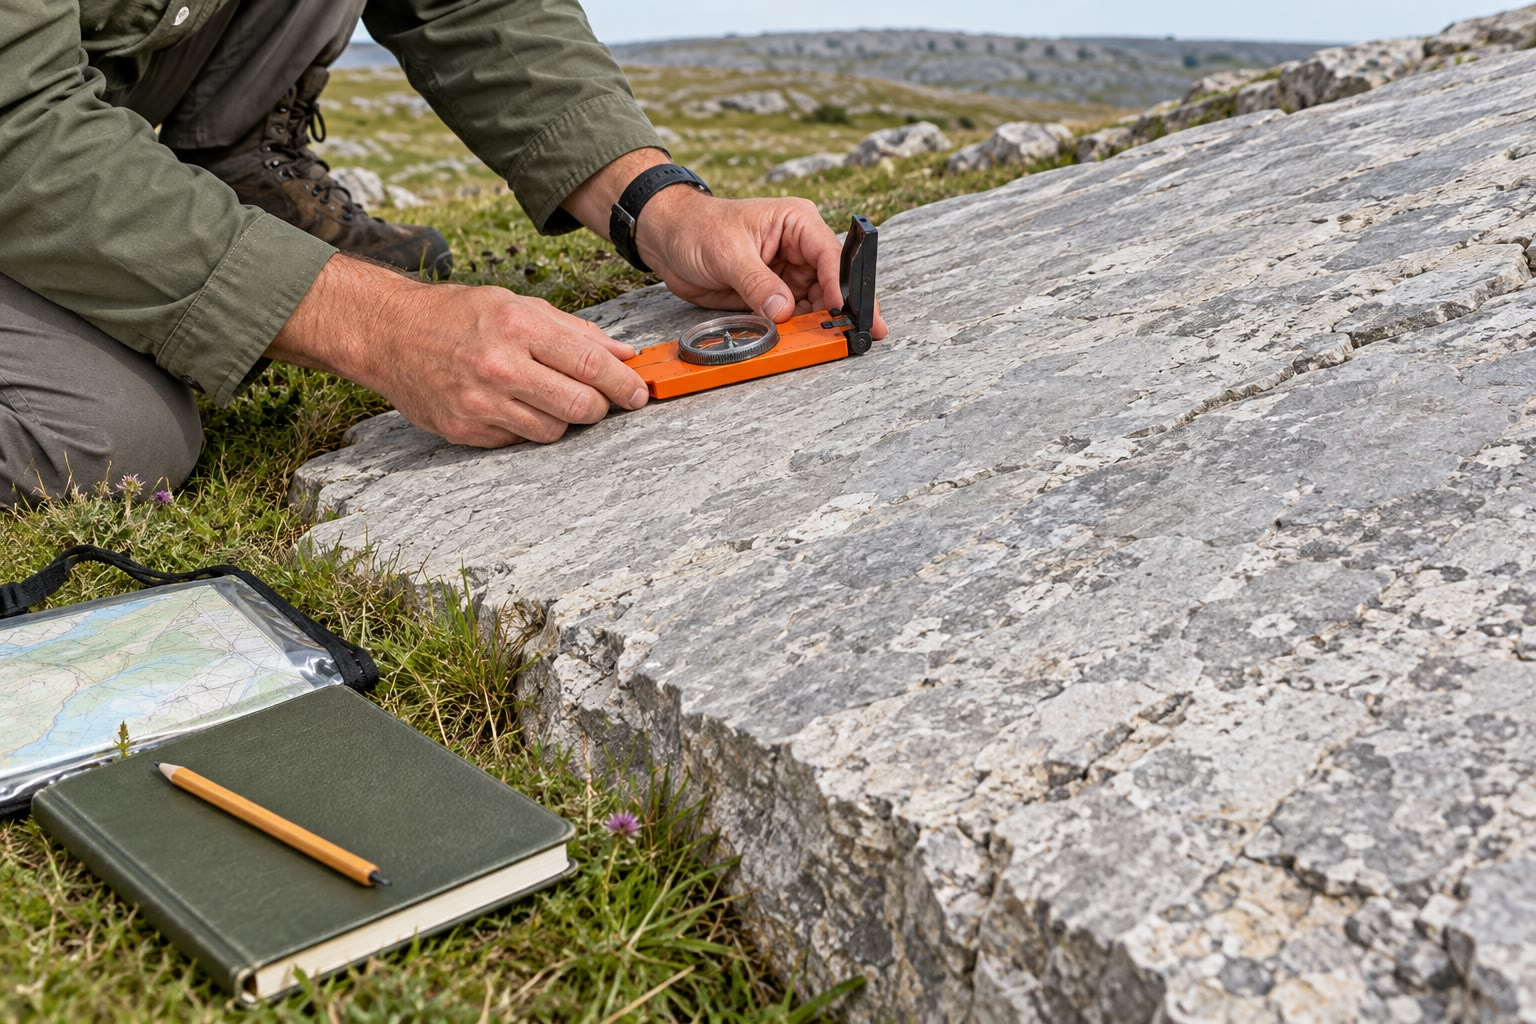
\includegraphics[width=0.6\linewidth]{images/book3/ai/b1-compass-clinometer.jpg}
\end{center}
\end{inthefield}

\begin{history}[किसी देश का पहला भूवैज्ञानिक मानचित्र]
% ledger: gsl:smith-1815, commons:smith-1815
सर्वेक्षक विलियम स्मिथ, जिसने इंग्लैंड में नहरें खोदीं और ज़मीन सुखाई, ने देखा कि शैल की हर परत अपने
जीवाश्म लिए होती है, और यह क्रम हर जगह एक-सा है। परतों को पहचानने के लिए जीवाश्मों का उपयोग करके उसने उन्हें
पंद्रह वर्षों से अधिक तक देश भर में अनुसरित किया। उसका मानचित्र, \emph{A Delineation of the Strata of England and
Wales, with part of Scotland}, जिस पर 1 अगस्त 1815 की तिथि है, किसी पूरे देश का पहला \omterm{def:b1:geological-maps:geological-map}{भूवैज्ञानिक मानचित्र} माना
जाता है।
\begin{center}
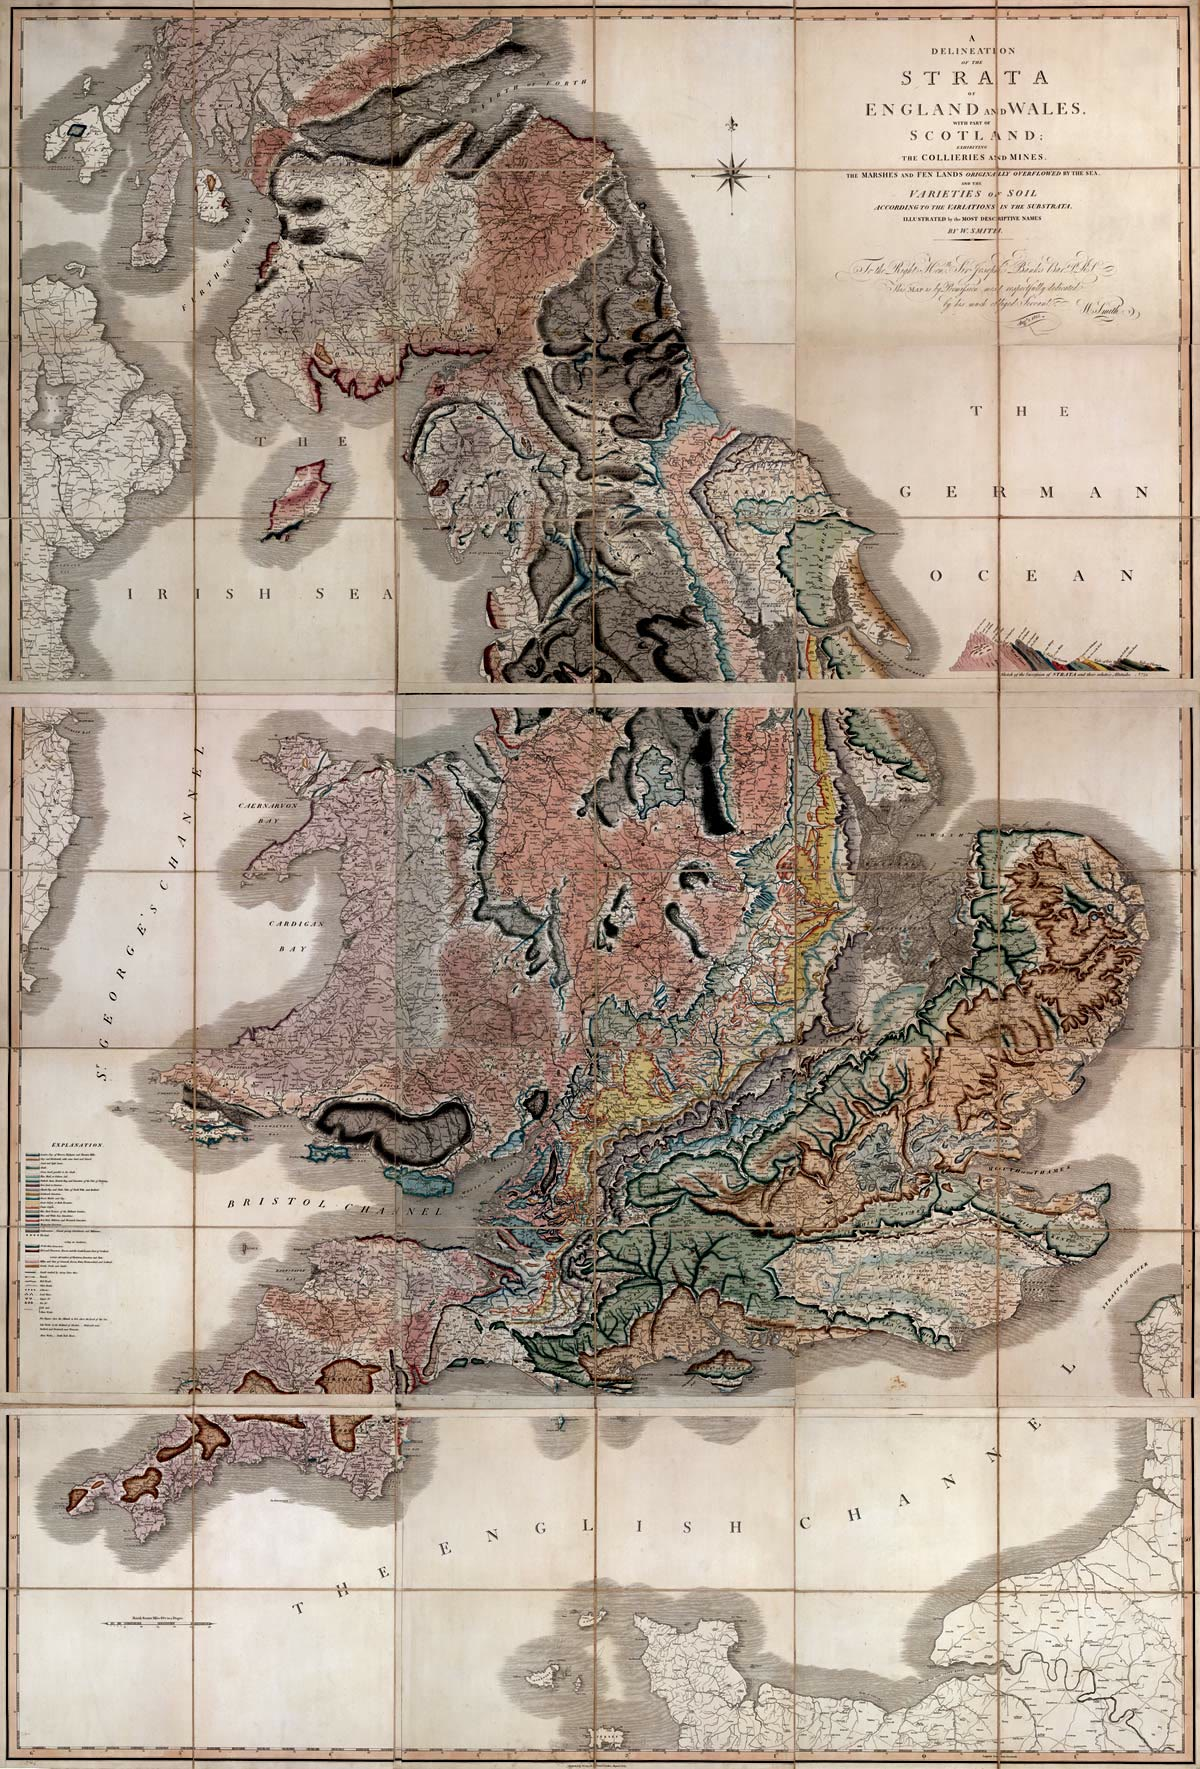
\includegraphics[width=0.36\linewidth]{images/book3/b1-smith-1815-map.jpg}

{\small विलियम स्मिथ का 1815 का मानचित्र (सार्वजनिक क्षेत्र)।}
\end{center}
\end{history}

\section{अभ्यास}

\begin{exercise}[$\star$]\label{exo:b1:geological-maps:1}
समतल का \omterm{def:b1:geological-maps:attitude}{स्ट्राइक}, \omterm{def:b1:geological-maps:attitude}{नति} और \omterm{def:b1:geological-maps:attitude}{नति-दिशा} परिभाषित कीजिए। एक शय्या का \omterm{def:b1:geological-maps:attitude}{अभिविन्यास} $135/40$ है: उसका \omterm{def:b1:geological-maps:attitude}{स्ट्राइक} दाएँ-हाथ
के नियम से दीजिए और उसका मानचित्र-चिह्न बनाइए।
\end{exercise}

\begin{exercise}[$\star$]\label{exo:b1:geological-maps:2}
\omterm{def:b1:geological-maps:attitude}{अभिविन्यास} $090/30$ वाले समतल का समीकरण लिखिए जो बिंदु $(0, 0, 500)$ से होकर जाता है, निर्देशांक मीटर में। वह $(1000, 0)$ और
$(0, 1000)$ पर किस उन्नयन पर है?
\end{exercise}

\begin{exercise}[$\star$]\label{exo:b1:geological-maps:3}
एक मानचित्र पर एक \omterm{def:b1:geological-maps:geological-map}{संपर्क} का अनुरेख कई किलोमीटर की पहाड़ियों और घाटियों पर \qty{350}{m} की समोच्च रेखा का
ठीक अनुसरण करता है। \omterm{def:b1:geological-maps:geological-map}{संपर्क} के बारे में आप क्या कह सकते हैं? और यदि उसका अनुरेख पहाड़ियों और घाटियों के आरपार एक
सीधी रेखा हो?
\end{exercise}

\begin{exercise}[$\star$]\label{exo:b1:geological-maps:4}
वार्डन पहाड़ियों के मानचित्र पर, नदी के किनारे वाली \omterm{def:b1:geological-maps:fold}{अपनति} के क्रोड में कौन-सी इकाई \omterm{def:b1:geological-maps:geological-map}{बहिर्भाग} बनाती है, और \omterm{def:b1:geological-maps:fold}{अभिनति}
के क्रोड में कौन-सी इकाई है? अध्यारोपण के सिद्धांत से समझाइए कि ऐसा क्यों है।
\end{exercise}

\begin{exercise}[$\star\star$]\label{exo:b1:geological-maps:5}
एक \omterm{def:b1:geological-maps:geological-map}{संपर्क} $\qty{300}{m}$ उन्नयन पर $(0, 0)$ पर, $\qty{300}{m}$ पर $(1000, 0)$ पर और $\qty{200}{m}$ पर $(0, 500)$ पर मिलता है
(मीटर, $x$ पूर्व, $y$ उत्तर)। उसका \omterm{def:b1:geological-maps:attitude}{स्ट्राइक}, \omterm{def:b1:geological-maps:attitude}{नति-दिशा} और \omterm{def:b1:geological-maps:attitude}{नति} ज्ञात कीजिए, पहले संरचना समोच्चों पर
तर्क करके, फिर \cref{thm:b1:geological-maps:three-point} से।
\end{exercise}

\begin{exercise}[$\star\star$]\label{exo:b1:geological-maps:6}
एक घाटी का तल उत्तर की ओर \qty{30}{m} प्रति km नीचे उतरता है। यदि एक \omterm{def:b1:geological-maps:geological-map}{संपर्क} (क) क्षैतिज है; (ख)
\ang{20} दक्षिण की ओर झुकता है; (ग) \ang{1} उत्तर की ओर झुकता है; (घ) \ang{20} उत्तर की ओर झुकता है, तो उसके \omterm{def:b1:geological-maps:geological-map}{बहिर्भाग}
का V किस ओर इंगित करता है? \cref{thm:b1:geological-maps:v-rule} से उचित ठहराइए।
\end{exercise}

\begin{exercise}[$\star\star$]\label{exo:b1:geological-maps:7}
V-नियम की स्थिति में, एक \omterm{def:b1:geological-maps:geological-map}{संपर्क} $a = 0.364$ (\ang{20}) के साथ प्रवाह की दिशा में झुकता है, और घाटी का तल $s = 0.03$
के साथ नीचे उतरता है। घाटी के एक किनारे का एक बिंदु तल से \qty{80}{m} ऊँचा है। उस बिंदु पर अनुरेख शीर्ष के कितना
ऊपर-प्रवाह में है?
\end{exercise}

\begin{exercise}[$\star\star$]\label{exo:b1:geological-maps:8}
वार्डन \omterm{def:b1:geological-maps:fold}{अपनति} के \omterm{def:b1:geological-maps:geological-map}{बहिर्भाग} उसके क्रोड के उत्तरी सिरे के चारों ओर बंद होते हैं। \omterm{def:b1:geological-maps:fold}{वलन-अक्ष} किस दिशा में नमन करता है?
क्या \omterm{def:b1:geological-maps:fold}{अभिनति} के \omterm{def:b1:geological-maps:geological-map}{बहिर्भाग} उत्तर की ओर बंद होंगे या दक्षिण की ओर?
\end{exercise}

\begin{exercise}[$\star\star$]\label{exo:b1:geological-maps:9}
\omterm{def:b1:geological-maps:geological-map}{भूवैज्ञानिक मानचित्र} पर, भ्रंश के अनुदिश, कौन-सी ओर सतह पर नई इकाइयाँ दिखाती है? कौन-सा खंड नीचे खिसका? भ्रंश-चिह्न से
जाँचिए।
\end{exercise}

\begin{exercise}[$\star\star\star$]\label{exo:b1:geological-maps:10}
दिखाइए कि \omterm{def:b1:geological-maps:attitude}{अभिविन्यास} $(\alpha_1, \delta_1)$ और $(\alpha_2, \delta_2)$ वाले दो समतल एक ऐसी रेखा के अनुदिश प्रतिच्छेद
करते हैं जो $\vec n_1 \times \vec n_2$ के समांतर है, जहाँ $\vec n_i = (\tan\delta_i\sin\alpha_i,
\tan\delta_i\cos\alpha_i, 1)$। इसे समतलों $090/30$ और $270/30$ पर लागू कीजिए: वह रेखा क्या है, और दोनों समतल किस
प्रकार का \omterm{def:b1:geological-maps:fold}{वलन} बनाते हैं?
\end{exercise}

\begin{exercise}[$\star\star\star$]\label{exo:b1:geological-maps:11}
एक ऊर्ध्वाधर डाइक \ang{045} \omterm{def:b1:geological-maps:attitude}{स्ट्राइक} करता है और मूल-बिंदु पर, \qty{0}{m} उन्नयन वाली घाटी के तल पर, \omterm{def:b1:geological-maps:geological-map}{बहिर्भाग}
बनाता है। \qty{300}{m} की एक पहाड़ी पर उसका अनुरेख कहाँ हो सकता है? एक दूसरे डाइक का वही \omterm{def:b1:geological-maps:attitude}{स्ट्राइक} है, वह
दक्षिण-पूर्व की ओर \ang{60} झुकता है और वह भी मूल-बिंदु पर \omterm{def:b1:geological-maps:geological-map}{बहिर्भाग} बनाता है। \qty{300}{m} की ज़मीन पर उसका
अनुरेख मूल-बिंदु से कितनी दूर और किस दिशा में है, \omterm{def:b1:geological-maps:attitude}{स्ट्राइक} के लंबवत मापा गया?
\end{exercise}

\begin{exercise}[$\star\star\star$]\label{exo:b1:geological-maps:12}
\qty{100}{m} के ग्रिड वाले एक \omterm{def:b1:geological-maps:dem}{अंकीय उन्नयन मॉडल} में, $(x, y)$ और $(x + 100, y)$ पर ज़मीन \qty{420}{m} और
\qty{405}{m} पर है, और $(x, y + 100)$ पर \qty{412}{m} पर। उस वर्ग-कोष्ठ में ज़मीन को एक समतल मानकर उसकी ढलान (डिग्री में)
और वह दिगंश परिकलित कीजिए जिस ओर वह मुँह करती है (नीचे-ढलान की दिशा)।
\end{exercise}

\section{समस्या: वार्डन पहाड़ियों को हल करना}

\begin{problem}[{सप्ताहांत समस्या --- बोरहोलों और एक मानचित्र से वलन-अक्ष, भ्रंश और एक क्षेत्र के इतिहास तक}]
\label{pb:b1:geological-maps:1}
% all data computed in figdata/bachelor-1/varden_maps.py from the region's
% model (figdata/shared/region.py); invented region: exercise data, no ledger
एक कंपनी, जो पेयजल के लिए वार्डन पहाड़ियों में बोरहोल खोद रही है, दर्ज करती है कि उसके बोरहोल चूना-पत्थर
के आधार से कहाँ मिलते हैं; उसके भूवैज्ञानिक भ्रंश को भी वहाँ ढूँढते हैं जहाँ वह ज़मीन को पार करता है। निर्देशांक
मानचित्र के दक्षिण-पश्चिम कोने से पूर्व और उत्तर में मीटरों में हैं; उन्नयन समुद्र तल से ऊपर मीटरों में हैं। भाग I
मानचित्र के रंगीन \omterm{def:b1:geological-maps:geological-map}{भूवैज्ञानिक मानचित्र}, \cref{sec:b1:geological-maps:cut}, का उपयोग करता है।
\medskip
\noindent\textbf{भाग I --- मानचित्र पढ़ना।}
\begin{enumerate}
  \item क्षेत्र की इकाइयाँ सबसे पुरानी से सबसे नई तक सूचीबद्ध कीजिए।
  \item नदी पश्चिम से पूर्व की ओर किन इकाइयों को काटती है?
  \item $x = \qty{3.5}{km}$ के पास \omterm{def:b1:geological-maps:fold}{वलन} के क्रोड में कौन-सी इकाई है? वह किस प्रकार का \omterm{def:b1:geological-maps:fold}{वलन} है?
  \item $x = \qty{7.5}{km}$ के पास \omterm{def:b1:geological-maps:fold}{वलन} के क्रोड में कौन-सी इकाई है? वह किस प्रकार का \omterm{def:b1:geological-maps:fold}{वलन} है?
  \item शिस्ट और ग्रेनाइट पहले \omterm{def:b1:geological-maps:fold}{वलन} के क्रोड में, केवल नदी के पास क्यों दिखते हैं?
  \item बलुआ पत्थर को ग्रेनाइट से कौन-सा \omterm{def:b1:geological-maps:geological-map}{संपर्क} अलग करता है? मानचित्र से उचित ठहराइए।
\end{enumerate}

\medskip
\noindent बोरहोल (चूना-पत्थर के आधार तक गहराई $d$ और ज़मीन का उन्नयन $z_g$) और वे तीन बिंदु F1--F3 जहाँ भ्रंश
आधार-चट्टान के शीर्ष को पार करता है (F2, घाटी में, पतली जलोढ़ के नीचे है, जिसे भ्रंश नहीं काटता):

\begin{omfigure}
\begin{minipage}[c]{0.42\linewidth}
\centering\small
\begin{tabular}{lrrrr}
\hline
 & पूर्व & उत्तर & $z_g$ & $d$ \\
\hline
E1 & 4000 & 6000 & 435 & 261 \\
E2 & 4600 & 7200 & 432 & 428 \\
E3 & 5100 & 6400 & 512 & 586 \\
W1 & 1500 & 6000 & 524 & 669 \\
W2 & 2200 & 7200 & 421 & 459 \\
W3 & 2600 & 5400 & 319 & 209 \\
\hline
 & पूर्व & उत्तर & $z_g$ & \\
\hline
F1 & 4197 & 1000 & 405 & \\
F2 & 5824 & 3500 & 129 & \\
F3 & 7321 & 6500 & 482 & \\
\hline
\end{tabular}
\end{minipage}\hfill
\begin{minipage}[c]{0.56\linewidth}
\centering
\begin{tikzpicture}
\begin{axis}[axis equal image, xmin=0, xmax=10, ymin=0, ymax=8, width=\linewidth,
  tick label style={font=\scriptsize}, xlabel={पूर्व (km)}, ylabel={उत्तर (km)},
  label style={font=\footnotesize}]
\addplot[fill=black!8, draw=black!50, line width=0.3pt, even odd rule] table {figdata/out/shared-region-unit-schist.dat};
\addplot[fill=black!8, draw=black!50, line width=0.3pt, even odd rule] table {figdata/out/shared-region-unit-granite.dat};
\addplot[fill=icsTriassic!20, draw=black!50, line width=0.3pt, even odd rule] table {figdata/out/shared-region-unit-sandstone.dat};
\addplot[fill=icsJurassic!25, draw=black!50, line width=0.3pt, even odd rule] table {figdata/out/shared-region-unit-limestone.dat};
\addplot[fill=icsJurassic!8, draw=black!50, line width=0.3pt, even odd rule] table {figdata/out/shared-region-unit-shale.dat};
\addplot[fill=icsCretaceous!20, draw=black!50, line width=0.3pt, even odd rule] table {figdata/out/shared-region-unit-chalk.dat};
\addplot[fault] table {figdata/out/shared-region-fault.dat};
\addplot[fill=omLithAlluv, draw=black!50, line width=0.3pt, even odd rule] table {figdata/out/shared-region-unit-alluvium.dat};
\addplot[river] table {figdata/out/shared-region-river.dat};
\addplot[only marks, mark=*, mark size=1.6pt] table[x=x_km, y=y_km] {figdata/out/bachelor-1-varden_maps-boreholes.dat};
\addplot[only marks, mark=square*, mark size=1.5pt, omThm] table[x=x_km, y=y_km] {figdata/out/bachelor-1-varden_maps-fault.dat};
\begin{scope}[every node/.style={font=\scriptsize\bfseries, inner sep=1.5pt, fill=white, fill opacity=0.8, text opacity=1}]
  \node[above right] at (axis cs:4,6) {E1};
  \node[above] at (axis cs:4.6,7.2) {E2};
  \node[right] at (axis cs:5.1,6.4) {E3};
  \node[above left] at (axis cs:1.5,6) {W1};
  \node[above] at (axis cs:2.2,7.2) {W2};
  \node[left] at (axis cs:2.6,5.4) {W3};
  \node[left, text=omThm] at (axis cs:4.197,1) {F1};
  \node[left, text=omThm] at (axis cs:5.824,3.5) {F2};
  \node[left, text=omThm] at (axis cs:7.321,6.5) {F3};
\end{scope}
\end{axis}
\end{tikzpicture}
\end{minipage}
\end{omfigure}

\medskip
\noindent\textbf{भाग II --- पूर्वी भुजा।}
\begin{enumerate}[resume]
  \item E1, E2 और E3 में चूना-पत्थर के आधार का उन्नयन परिकलित कीजिए।
  \item सदिश $\overrightarrow{E_1E_2}$ और $\overrightarrow{E_1E_3}$ लिखिए।
  \item उनका सदिश गुणनफल परिकलित कीजिए और उसे ऊपर की ओर अभिमुख कीजिए।
  \item पूर्वी भुजा पर चूना-पत्थर के आधार की \omterm{def:b1:geological-maps:attitude}{नति} निकालिए।
  \item उसकी \omterm{def:b1:geological-maps:attitude}{नति-दिशा} निकालिए, फिर दाएँ-हाथ के नियम से उसका \omterm{def:b1:geological-maps:attitude}{स्ट्राइक}।
  \item क्या परिणाम मानचित्र पर पूर्वी भुजा के स्ट्राइक-और-नति चिह्न से सुसंगत है?
\end{enumerate}

\medskip
\noindent\textbf{भाग III --- वलन।}
\begin{enumerate}[resume]
  \item W1, W2 और W3 में चूना-पत्थर के आधार के उन्नयन परिकलित कीजिए।
  \item पश्चिमी भुजा पर चूना-पत्थर के आधार का एक ऊर्ध्वमुखी अभिलंब $\vec n_W$ परिकलित कीजिए।
  \item पश्चिमी भुजा का \omterm{def:b1:geological-maps:attitude}{अभिविन्यास} निकालिए।
  \item दो भुजाओं के प्रतिच्छेद की एक दिशा, \omterm{def:b1:geological-maps:fold}{वलन-अक्ष}, $\vec n_E \times \vec n_W$ के रूप में परिकलित कीजिए (जहाँ $\vec n_E$ प्रश्न 9 से है)।
  \item \omterm{def:b1:geological-maps:fold}{वलन-अक्ष} की दिशा (उसके क्षैतिज प्रक्षेप का दिगंश, नीचे की ओर लिया गया) और नमन (क्षैतिज के नीचे उसका कोण) दीजिए।
  \item आधार का बलुआ पत्थर नदी के पार होने वाले स्थान पर $y = \qty{4}{km}$ के पास, अक्ष पर \qty{230}{m} पर है। \qty{8}{km}
        और उत्तर में अक्ष पर वह कितना नीचे है? क्या यह भाग I के प्रश्न 3 और बहिर्भागों के बंद होने से सुसंगत है?
\end{enumerate}

\medskip
\noindent\textbf{भाग IV --- भ्रंश और इतिहास।}
\begin{enumerate}[resume]
  \item F1, F2 और F3 से भ्रंश का \omterm{def:b1:geological-maps:attitude}{अभिविन्यास} परिकलित कीजिए।
  \item भ्रंश के अनुदिश, पूर्व-दक्षिण-पूर्व की ओर की सतह पर इकाइयाँ अपने सामने की इकाइयों से नई हैं। कौन-सा खंड
        नीचे खिसका? क्या भ्रंश सामान्य है या उत्क्रम?
  \item F1 से F3 तक की सीधी रेखा F2 से लगभग \qty{200}{m} पश्चिम से गुज़रती है। भ्रंश का अनुरेख नदी घाटी को पार करते
        समय, F2 पर, पूर्व-दक्षिण-पूर्व की ओर क्यों मुड़ता है?
  \item क्रम में लिखिए: \omterm{def:b1:geological-maps:fold}{वलन}; खड़िया का निक्षेपण; भ्रंशन; ग्रेनाइट का अंतर्वेधन; बलुआ पत्थर से पहले का अपरदन; जलोढ़ का
        निक्षेपण।
  \item खड़िया 90 मिलियन वर्ष पुरानी है और वलित है; जलोढ़ अंतिम 2.58 मिलियन वर्षों में बिछी
        और भ्रंशित नहीं है। \omterm{def:b1:geological-maps:fold}{वलन} और भ्रंशन किन आयुओं के बीच हुए?
  \item F1 के नीचे समुद्र तल से \qty{1000}{m} नीचे के भ्रंश तक पहुँचने के लिए F1 से कितनी दूरी पर और किस दिशा में एक ऊर्ध्वाधर कुआँ खोदना होगा?
\end{enumerate}
\end{problem}
